\documentclass[10pt]{article}
\usepackage[a4paper,margin=1.4cm]{geometry}
\usepackage{xcolor}
\usepackage[compat=1.1.0]{tikz-feynman}
\tikzfeynmanset{warn luatex=false}
\begin{document}
\section*{Top sectors as cut diagrams}
Amplitude (left) $\times$ conjugate (right) for $p_1 p_2 \to V(q)\, r_1 r_2 r_3$, glued along the cut (dashed): $r_1, r_2, r_3$ (blue), $q$ (red, $q^2 = m^2$). The rapidity condition $-q\cdot p_1 + u\, q\cdot p_2 = 0$ of every family is not a line. Internal lines carry their DD number. \textbf{Regular propagators} (DD numbers, all legs incoming): 6 = $(p_1+r_1)^2$; 7 = $(p_2+r_1)^2$; 8 = $(p_1+r_2)^2$; 9 = $(p_2+r_2)^2$; 10 = $(p_1+r_3)^2$; 11 = $(p_2+r_3)^2$; 12 = $(r_1+r_2)^2$; 13 = $(r_2+r_3)^2$; 14 = $(r_1+r_3)^2$; 15 = $(p_1+r_1+r_2)^2$; 16 = $(p_2+r_1+r_2)^2$; 17 = $(p_1+r_1+r_3)^2$; 18 = $(p_2+r_1+r_3)^2$; 19 = $(p_1+r_2+r_3)^2$; 20 = $(p_2+r_2+r_3)^2$; 21 = $(r_1+r_2+r_3)^2$; 22 = $(p_1+r_1+r_2+r_3)^2$; 23 = $(p_2+r_1+r_2+r_3)^2$; 24 = $(p_1+p_2+r_1)^2$; 25 = $(p_1+p_2+r_2)^2$; 26 = $(p_1+p_2+r_3)^2$; 27 = $(p_1+p_2+r_1+r_2)^2$; 28 = $(p_1+p_2+r_1+r_3)^2$; 29 = $(p_1+p_2+r_2+r_3)^2$.\par\medskip
\begin{minipage}[t]{0.48\textwidth}\centering\resizebox{0.9\linewidth}{!}{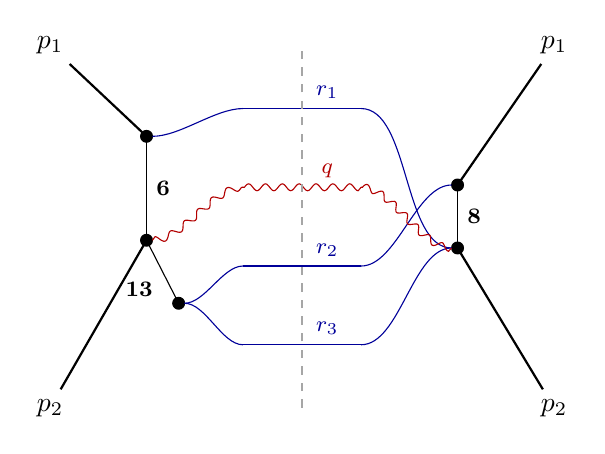
\begin{tikzpicture}
\begin{feynman}
\vertex (Lp1) at (-3.200,2.300) {$p_1$};
\vertex (Lp2) at (-3.200,-2.300) {$p_2$};
\vertex (Lcr1) at (-0.750,1.500);
\vertex (Lcr2) at (-0.750,-0.500);
\vertex (Lcr3) at (-0.750,-1.500);
\vertex (Lcq) at (-0.750,0.500);
\vertex[dot] (L6) at (-1.975,1.147) {};
\vertex[dot] (Lroot) at (-1.975,-0.173) {};
\vertex[dot] (L13) at (-1.567,-0.973) {};
\vertex (Rp1) at (3.200,2.300) {$p_1$};
\vertex (Rp2) at (3.200,-2.300) {$p_2$};
\vertex (Rcr1) at (0.750,1.500);
\vertex (Rcr2) at (0.750,-0.500);
\vertex (Rcr3) at (0.750,-1.500);
\vertex (Rcq) at (0.750,0.500);
\vertex[dot] (R8) at (1.975,0.529) {};
\vertex[dot] (Rroot) at (1.975,-0.271) {};
\diagram* {
(L6) -- [plain, edge label={\footnotesize\bfseries 6}] (Lroot),
(L13) -- [plain, edge label={\footnotesize\bfseries 13}] (Lroot),
(Lp1) -- [plain, thick] (L6),
(Lp2) -- [plain, thick] (Lroot),
(Lcr1) -- [plain, blue!60!black, out=180, in=0, looseness=0.75] (L6),
(Lcr2) -- [plain, blue!60!black, out=180, in=0, looseness=0.75] (L13),
(Lcr3) -- [plain, blue!60!black, out=180, in=0, looseness=0.75] (L13),
(Lcq) -- [boson, red!70!black, out=180, in=0, looseness=0.75] (Lroot),
(R8) -- [plain, edge label={\footnotesize\bfseries 8}] (Rroot),
(Rp1) -- [plain, thick] (R8),
(Rp2) -- [plain, thick] (Rroot),
(Rcr1) -- [plain, blue!60!black, out=0, in=180, looseness=0.75] (Rroot),
(Rcr2) -- [plain, blue!60!black, out=0, in=180, looseness=0.75] (R8),
(Rcr3) -- [plain, blue!60!black, out=0, in=180, looseness=0.75] (Rroot),
(Rcq) -- [boson, red!70!black, out=0, in=180, looseness=0.75] (Rroot),
(Lcr1) -- [plain, blue!60!black] (Rcr1),
(Lcr2) -- [plain, blue!60!black] (Rcr2),
(Lcr3) -- [plain, blue!60!black] (Rcr3),
(Lcq) -- [boson, red!70!black] (Rcq),
};
\end{feynman}
\draw[dashed, gray!70] (0,-2.30) -- (0,2.30);
\node[font=\footnotesize, blue!60!black, above] at (0.32,1.50) {$r_1$};
\node[font=\footnotesize, blue!60!black, above] at (0.32,-0.50) {$r_2$};
\node[font=\footnotesize, blue!60!black, above] at (0.32,-1.50) {$r_3$};
\node[font=\footnotesize, red!70!black, above] at (0.32,0.50) {$q$};
\end{tikzpicture}}\\[2mm]\textbf{FAM[55]} (topo55), sector with 3 of 7 lines\\[2pt]{\footnotesize\begin{tabular}{@{}r@{\ \ }l@{\ \ }l@{}}\textbf{6} & $(p_1+r_1)^2$ & amplitude\\
\textbf{13} & $(r_2+r_3)^2$ & amplitude\\
\textbf{8} & $(p_1+r_2)^2$ & conjugate\\\end{tabular}}\\[2pt]{\scriptsize pinched: 7 = $(p_2+r_1)^2$, 14 = $(r_1+r_3)^2$, 18 = $(p_2+r_1+r_3)^2$, 22 = $(p_1+r_1+r_2+r_3)^2$}\end{minipage}\hfill%
\end{document}